\hypertarget{distributed-systems}{%
\section{Distributed systems}\label{distributed-systems}}

We implement distributed systems when our system becomes too big to be
run from a single computer. Distribution always makes things more
complex, so there is no reason to implement it when you don't have to.
But in almost every case, you eventually will.

Most of the following text is based on
\href{https://disco.ethz.ch/courses/podc_allstars/lecture/chapter17.pdf}{this
lecture series} and this
\href{https://towardsdatascience.com/distributed-transactions-and-why-you-should-care-116b6da8d72}{blog
bost for overall context}.

An interesting note: distributed systems are really only complicated
when the peers have state. If all but one node are stateless, we talk of
a `microservice-architecture', which has none of the pitfalls of other
distributed systems (except logging: maybe put all logs in one central
database). Riesgos is one example of such an architecture. There, the
worst thing you have to deal with is unresponsive micro-services.

\hypertarget{acid}{%
\subsection{ACID}\label{acid}}

A transaction is a sequence of database operations that can be
considered one independent, coherent unit of work. A database
transaction should have the ACID-properties: - Atomicity: Transactions
are often composed of multiple statements. Atomicity guarantees that
each transaction is treated as a single ``unit'', which either succeeds
completely, or fails completely. - Consistency: All nodes must see the
same results of an operation at any given time - Isolation: Each
Transaction must proceed as if it were the only one - Durability: All
state changes must be persistent upon commit

Use ACID datastorage when you really need consistency, and when just
eventual consistency is not enough. You need ACID in banking, except
credit cards, which can handle eventual consistency.

\hypertarget{theorems}{%
\subsection{Theorems}\label{theorems}}

\hypertarget{flp-theorem}{%
\subsubsection{FLP theorem}\label{flp-theorem}}

We will prove that there is no algorithm which, for all possible
sequences of events, always reaches a point in time \(t\) such that the
configuration \(C_t\) is decided.

\[ !\exists \text{alg}: \forall s \exists t: C_t:\text{unival}   \]
Proof by contradiction.

\hypertarget{definitions}{%
\paragraph{Definitions}\label{definitions}}

\begin{itemize}
 
\item
  \(C\): a system configuration
\item
  \(e = (m, p)\): an event, consisting of a message \(m\) and a
  receiving process \(p\)
\item
  \(s = [(m_0, p_0), (m_1, p_1), ...]\): a sequence of events
\item
  \(C:\text{unival}\): a configuration from which any sequence of events
  can only lead to one outcome.
\item
  \(C:\text{bival}\): a configuration from which different sequences may
  still lead to different outcomes (in other words, a configuration that
  is still undecided).
\end{itemize}

\hypertarget{lemma-1-disjoint-sequences-are-commutative.}{%
\paragraph{Lemma 1: Disjoint sequences are
commutative.}\label{lemma-1-disjoint-sequences-are-commutative.}}

Let \(p_{s_1}\) be the list of all the processes that occur in the
sequence \(s_1\) \[ 
      p_{s_1} \cap p_{s_2} = \{\} \to C \odot s_1 \odot s_2 = C \odot s_2 \odot s_1
\] If the sequences of messages \(s_1\) and \(s_2\) have no common
processes, than they may be applied to a configuration \(C\) in any
order and will yield the same result.

\hypertarget{lemma-2-there-is-always-a-bivalent-initial-configuration}{%
\paragraph{Lemma 2: There is always a bivalent initial
configuration}\label{lemma-2-there-is-always-a-bivalent-initial-configuration}}

\[
\forall \text{alg}: \exists C:\text{bival}
\] Proof by contradiction. Assume \[
\exists \text{alg}: \forall C:\text{unival}
\]

Consider a few known configurations. - \(C_0 = [0, 0, ..., 0]\) must be
univalent-0 - \(C_{2^n} = [1, 1, ..., 1]\) must be univalent-1

Thus, the set of all initial configurations contains both univalent-0
and univalent-1 configurations.

Also, all configurations are in a neighborhood-tree with only one
process-suggestion between neighbors.

Thus:

\[
\exists C_i:\text{unival-0} \\
\land \exists C_{i+1}, \exists p: C_{i+1} = C_i \odot \text{flip}(p) \\
\land C_{i+1}:\text{unival-1}
\]

There must be some process \(C_i:\text{unival-0}\) which is an immediate
neighbor of a \(C_{i+1}:\text{unival-1}\) which differs from \(C_i\) in
just one process \(p\) initially suggesting differently.

Now suppose that \(p\) fails immediately. Then:

\[
C_i \odot \text{fail}(p) = C_{i+1} \odot \text{fail}(p)
\] Thus \[
\forall s: C_i \odot \text{fail}(p) \odot s = C_{i+1} \odot \text{fail}(p) \odot s
\] But this contradicts the statement that \[
C_i:\text{unival-0} \\
\land C_{i+1}:\text{unival-1}
\]

Thus, there \emph{must} be some \(C:\text{bival}\), that is some initial
configuration that is bi-valent.

\hypertarget{lemma-3-there-is-always-a-sequence-that-can-lead-from-one-bivalent-state-to-another}{%
\paragraph{Lemma 3: There is always a sequence that can lead from one
bivalent state to
another}\label{lemma-3-there-is-always-a-sequence-that-can-lead-from-one-bivalent-state-to-another}}

With this lemma, we will have proven that there is a sequence that
cannot be deciding, and therefore have proven the FLP-impossibility.

\[
C^*:\text{bival} \to \exists s: C^* \odot s: \text{bival} \\
\]

Consider a bi-valent configuration \(C^*\) and some so-called
\emph{deciding} event \(e\). Consider two sets: -
\(\mathbb{C} := \{ C | C = C^* \odot s \land e \notin s \}\) -
\(\mathbb{D} := \{ D | D = C \odot e \land C \in \mathbb{C} \}\)



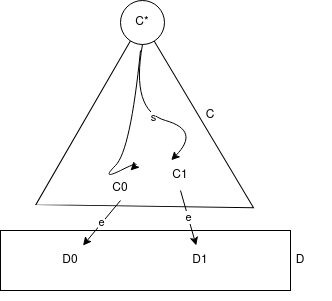
\includegraphics{images/flp_sets_c_d.png}


Then lemma 3 can be reformulated as: \[
C^*:\text{bival} \to \exists s: C^* \odot s: \text{bival} \\
\equiv \exists D \in \mathbb{D}: D:\text{bival}
\]

Proof by contradiction. Assume that \[
\forall D \in \mathbb{D}: D:\text{unival}
\]

\hypertarget{lemma-3.1-there-is-a-0-valent-and-a-1-valent-configuration-in-mathbbd}{%
\paragraph{\texorpdfstring{Lemma 3.1: There is a 0-valent and a 1-valent
configuration in
\(\mathbb{D}\)}{Lemma 3.1: There is a 0-valent and a 1-valent configuration in \textbackslash mathbb\{D\}}}\label{lemma-3.1-there-is-a-0-valent-and-a-1-valent-configuration-in-mathbbd}}

We initially assumed that \(\exists \text{alg}: \text{correct}\). That
means that even though \(C^*:\text{bival}\), eventually all paths from
\(C^*\) must be univalent. Also, since \(C^*:\text{bival}\), there must
be a univalent-0 and a univalent-1 configuration.

Thus: $ \exists E\_0: \text{unival-0} $

\begin{itemize}
 
\item
  Case 1: \(E_0 \in \mathbb{C}\)

  \begin{itemize}
   
  \item
    Let \(F_0 = E_0 \odot e\)
  \item
    Then \(F_0 \in \mathbb{D} \land F_0:\text{unival-0}\)
  \end{itemize}
\item
  Case 2: \(E_0 \notin \mathbb{C}\)

  \begin{itemize}
   
  \item
    \(\exists F_0 \in \mathbb{D}: \exists s: E_0 = F_0 \odot s\)
  \item
    Then \(F_0 \in \mathbb{D} \land F_0:\text{unival-0}\)
  \end{itemize}
\end{itemize}

\begin{figure}
\caption{Case 1}
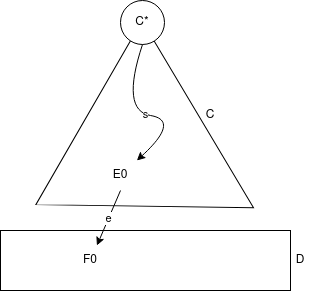
\includegraphics{images/flp_e0_f0.png}
\end{figure}

\begin{figure}
\caption{Case 2}
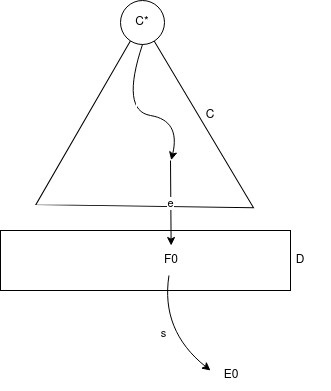
\includegraphics{images/flp_f0_e0.png}
\end{figure}

By the same logic: \[
\exists E_1: \text{unival-1} \\
\land \exists F_1 \in \mathbb{D}: F_1: \text{unival-1}
\]

\hypertarget{lemma-3.2-there-are-two-neighbors-in-mathbbc-that-lead-to-differently-valent-members-of-mathbbd}{%
\paragraph{\texorpdfstring{Lemma 3.2: There are two neighbors in
\(\mathbb{C}\) that lead to differently-valent members of
\(\mathbb{D}\)}{Lemma 3.2: There are two neighbors in \textbackslash mathbb\{C\} that lead to differently-valent members of \textbackslash mathbb\{D\}}}\label{lemma-3.2-there-are-two-neighbors-in-mathbbc-that-lead-to-differently-valent-members-of-mathbbd}}

All configurations in \(\mathbb{C}\) are in a neighborhood-tree: \[
\forall C \in \mathbb{C} \setminus C^*: \exists C' \in \mathbb{C}: \exists e': C = C' \odot e'
\]

From lemma 3.1 we know that -
\(\exists D_0 \in \mathbb{D}: D_0:\text{unival-0}\) -
\(\exists D_1 \in \mathbb{D}: D_1:\text{unival-1}\)

Together: \[
\exists C_0, C_1 \in \mathbb{C}: C_1 = C_0 \odot e' \\
\land (C_0 \odot e):\text{unival-0} \\
\land (C_1 \odot e):\text{unival-1}
\]

\hypertarget{lemma-3.3-if-p-neq-p-this-leads-to-a-contradiction}{%
\paragraph{\texorpdfstring{Lemma 3.3: If \(p \neq p'\) this leads to a
contradiction}{Lemma 3.3: If p \textbackslash neq p' this leads to a contradiction}}\label{lemma-3.3-if-p-neq-p-this-leads-to-a-contradiction}}

If \(e' = (m', p')\) and \(e = (m, p)\) and \(p \neq p'\), then we can
apply lemma 1 to the two sequences \(s_1 = [e', e]\) and
\(s_2 = [e, e']\).

With this, we have \(C_0 \odot s_1 = C_0 \odot s_2 = D_1\)

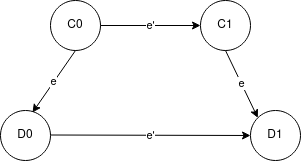
\includegraphics{images/flp_lemma_33.png}


We know from lemma 3.2 that \(D_0:\text{unival-0}\), thus all events
starting from \(D_0\) can only lead to another \(\text{unival-0}\)
configuration. But we also know that \(D_1:\text{unival-1}\) - and
\(D_1\) can be reached from \(D_0\) via \(e'\). A contradiction.

\hypertarget{lemma-3.4-if-p-p-this-leads-to-a-contradiction}{%
\paragraph{\texorpdfstring{Lemma 3.4: If \(p = p'\) this leads to a
contradiction}{Lemma 3.4: If p = p' this leads to a contradiction}}\label{lemma-3.4-if-p-p-this-leads-to-a-contradiction}}

Let \(s\) be a deciding sequence in which \(p\) plays no part. There is
a deciding run, because we assumed that our algorithm is always correct.

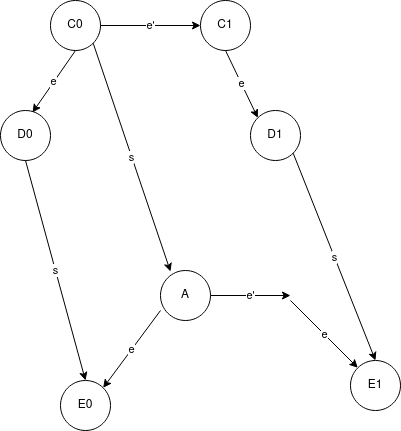
\includegraphics{images/flp_lemma_34.png}


As we can see in the graphic, \(A\) is bivalent, because we can move to
both \(E_0\) and \(E_1\) from \(A\). But \(s\) was supposed to be a
deciding run, so \(A\) must be univalent. Again, this is a
contradiction.

\begin{quote}
Thus, there is always a sequence that cannot be deciding. That means
that there is no algorithm which always reaches a deciding state at some
point for \emph{all} possible sequences.
\end{quote}

\hypertarget{interpretation-of-flp-impossibility}{%
\paragraph{Interpretation of
FLP-impossibility}\label{interpretation-of-flp-impossibility}}

Really FLP proves that of failure-tolerance, termination and agreement
all consensus-algorithms must chose at most 2.

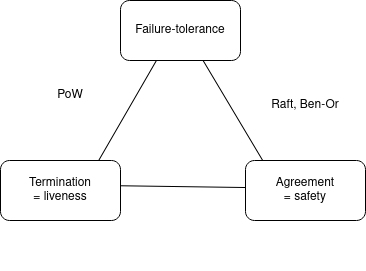
\includegraphics{images/flp_triangle.png}


Especially, termination is often replaced to
\(P(\text{termination}) \approx 1\). That is what raft and ben-or do.
The worst enemy of consensus is a Byzantine network that always delays
and delivers the exact wrong message. By randomizing the consensus, even
an evil network only has a small chance to find the right message to
delay\ldots{} and that chance gets ever smaller with each iteration.

\hypertarget{cap-theorem}{%
\subsubsection{CAP-Theorem}\label{cap-theorem}}

There are nowadays no \emph{distributed} databases that are not
partition tolerant - it is illusionary to assume that a network cannot
be partitioned. (However, if your database will always stay on one
machine only, feel free to design for CA) If a distributed database
provides the acid-properties, then it must chose consistency (CP) over
availability (AP) according to the cap theorem. An available (AP)
database cannot provide acid-transactions.

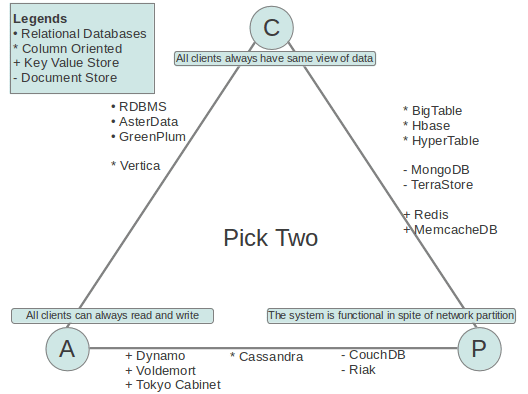
\includegraphics{images/cap_triangle.png}


Just as in the FLP-triangle we relaxed termination to probabilistic
termination, in CAP we commonly replace consistency with eventual
consistency.

\hypertarget{crdts}{%
\paragraph{CRDTs}\label{crdts}}

A neat way to achieve eventual consistency are CRDTS, set-based
databases that automatically correct themselves on reads. They are
useful because they achieve consistency without the need for a consensus
algorithm. Instead of consensus, writes always happen immediately. If a
node lags behind, the difference is detected and overwritten. Data is
append-only.

\hypertarget{byzantine-agreement}{%
\subsubsection{Byzantine agreement}\label{byzantine-agreement}}

In the FLP-theorem, we considered the so-called `crash'-mode of process
failure, where a process stops responding. This is not the worst kind of
error, though. Byzantine errors are those where a node actively tries to
sabotage the consensus-process.

Imagine three Byzantine generals laying siege to an enemy city. They
have to decide if they want to attack the city or not. An attack can
only be successful if they all attack together, so they must agree on
attack or abstain together. Each general has his own information on
whether an attack, even with all three generals involved, will be
successful or not. Finally, there is a traitor among them, who will do
everything he can to make them decide on the wrong strategy. The two
loyal (a.k.a. \emph{correct}) generals follow some algorithm (like
e.g.~majority-vote, or seniority) for making their decision, while the
traitor will do anything he wants. For Byzantine agreement to be
possible, the following must hold:

\begin{itemize}
 
\item
  \emph{Agreement}: The two loyal generals decide upon the same value,
  that is, whether to attack or not.
\item
  \emph{Validity}: The decision is made soundly. If both generals think
  its a good idea to attack, the agreement must be on `attack'; if both
  think that it isn't, then the agreement must be on `abstain'. If one
  general thinks an attack would be smart while the other doesn't, this
  rule doesn't hold, and only item 1 holds.
\end{itemize}

In other words, if Byzantine agreement were possible, it would mean that
there is an approach where one traitor cannot make the generals choose a
bad strategy. However, we will proof that Byzantine agreement is
\emph{not} possible.

We can easily proof this. We have three nodes \(u\),\(v\),\(w\). In
order to achieve validity, a correct node must decide on its own value
if another node supports that value.The third node might disagree, but
that node could be a traitor. If correct node \(u\) has input 0 and
correct node \(v\) has input 1, the Byzantine node \(w\) can fool them
by telling \(u\) that its value is 0 and simultaneously telling \(v\)
that its value is 1. This leads to \(u\) and \(v\) deciding on their own
values, which results in violating the agreement condition. Even if
\(u\) talks to \(v\), and they figure out that they have different
assumptions about \(w\)'s value, \(u\) cannot distinguish whether \(w\)
or \(v\) is a traitor.

\hypertarget{consensus-algorithms}{%
\subsection{Consensus algorithms}\label{consensus-algorithms}}

Consensus is the process by which multiple nodes agree on a single
result to guarantee consistency among them. Therefore, consensus
prodvides the `C' in `ACID'.

Consensus requires - agreement: all nodes accept the final result -
validity: the final result was one of the proposed options -
termination: unlike Belgium, you must not be stuck in stalemate forever

By the FLP-theorem \emph{no asynchronous protocol can always reach
consensus in a bounded time, in the event of even a single node
failure}. But the below algorithms achieve consensus in most situations.

\hypertarget{two-phase-commit}{%
\subsubsection{Two-phase commit}\label{two-phase-commit}}

One of the simplest consensus-algorithms. Perhaps one of the most widely
used distributed consensus algorithms, this contains two phases --- The
Voting Phase and the Commit phase. In the voting phase, the transaction
manager asks every node for the result, then decides the correct value
based on majority consensus and gives it back to the nodes. If everyone
agrees, the transaction manager contacts every participants again to let
them know about the final value. Otherwise, contact every participant to
abort the consensus. The participants do not have to agree on a value
but have to agree on whether or not to agree on the value provided by
the Transaction manager.

\hypertarget{raft}{%
\subsubsection{Raft}\label{raft}}

Raft is an algorithm to pick one leader out of all peers. It facilitates
a CP-system. It is a special type of two-phase-commit algorithm.

\begin{itemize}
 
\item
  Metadata: each node has\ldots{} - role: `follower' \textbar{}
  `candidate' \textbar{} `leader' - election-timeout: int (random
  between 150-300ms) - election-term: int
\item
  Leader selection - All nodes initially are followers - If a node
  doesn't hear the heartbeat from the leader for a while, it becomes a
  candidate and starts a new election-term. - A candidate votes for
  itself and requests votes from all other nodes - Nodes that receive a
  ``vote for me'' for the first time increment their election-term, too.
  They also reset their election-timeout. If they haven't received any
  ``vote for me'' during the ongoing therm, they reply with a ``yes'' -
  The node with a \textbf{majority} votes will now start sending out a
  heartbeat to all followers. - In case of a draw - two nodes having the
  same amount of votes - no majority is present. One node will time-out
  first and start a new election.
\item
  Data commit through log-replication - All data-changes now go through
  leader - Leader earmarks a change and broadcasts ``earmark change'' to
  followers - When a \textbf{majority} of followers have responded with
  ``ACK - change earmarked'', the leader commits the change himself -
  The leader now broadcasts ``commit change'' to all followers -
  Earmark- and commit-messages also count as heartbeat.
\end{itemize}

\hypertarget{raft---partition-tolerance}{%
\paragraph{Raft - partition
tolerance}\label{raft---partition-tolerance}}

A commit to the smaller halve of a partition will never be accepted,
because the leader of that partition never gets a majority-ACK. Commits
to the larger partition will go through, though. Upon re-connection, the
older leader (the one with the lower election-term) will step down. All
its followers will unroll uncommited logs and instead match the newer
leaders log.

\hypertarget{byzantine-fault-tolerance}{%
\paragraph{Byzantine fault tolerance}\label{byzantine-fault-tolerance}}

Raft is not a Byzantine fault tolerant algorithm: the nodes trust the
elected leader.

\hypertarget{paxos}{%
\subsubsection{Paxos}\label{paxos}}

Paxos is a ridiculously complicated consensus algorithm. It's a
three-phase-commit algorithm. Reference
\href{http://lamport.azurewebsites.net/pubs/pubs.html\#lamport-paxos}{here}

PAXOS is a method of achieving consensus in a network with unreliable
nodes. It contains the following roles --- a Client which issues a
request to the distributed system, Acceptors which form a quorum, a
Proposer is an advocate for the client request trying to convince
acceptors to accept it, a learner takes action once a request has been
accepted, a leader is who is also a Distinguished Proposer and a
Distinguished Learner. The leader then chooses the ``valid result'' and
sends it to all the nodes, the nodes can reply with an accept or a
reject. If a majority of nodes accept then the value is committed.
Apache Zookeeper and Google Spanner use the PAXOS algorithm to achieve
consensus.

\hypertarget{byzantine-fault-tolerance-1}{%
\paragraph{Byzantine fault
tolerance}\label{byzantine-fault-tolerance-1}}

Paxos is not a Byzantine fault tolerant algorithm.

\hypertarget{bitcoin}{%
\subsubsection{Bitcoin}\label{bitcoin}}

Bitcoin is an AP database/log. It is eventually consistent.

A block contains - the previous blocks hash - a few transactions - a
running id - source, target, quantity - signature of source - a value
that would make this blocks hash all zeros

There are special users called miners. Miners collect outstanding
transactions, add them to a block, solve the hash-riddle, and broadcast
the freshly verified block to everyone who's currently online. Miners
are in a race with each other: the first miner to verify and broadcast a
block gets a reward in the form of a few bitcoin. All others, who have
already started working, now must: - replace their blocks
\texttt{previousHash} value with the latest one - replace any
transactions in their block that have already been commited - solve the
hash-riddle again

This means that your transaction may be rejected several times until it
is part of one block that is actually accepted. (Note that this does not
happen in proof of stake-validation, because there only one person does
the work)

\hypertarget{bitcoin-partition-tolerance-and-eventual-consistency}{%
\paragraph{Bitcoin partition tolerance and eventual
consistency}\label{bitcoin-partition-tolerance-and-eventual-consistency}}

If there is a network partition, the blockchain may diverge. Upon
re-connection, each peer choses the longest chain. All blocks that have
been commited on the shorter chain are considered invalid and their
transactions will have to be re-done in new blocks. For this reasons,
banks don't trust a block until it is at least a few levels deep in the
chain (the longest block-revert in history was 24 blocks).

\hypertarget{proof-of-stake}{%
\paragraph{Proof of stake}\label{proof-of-stake}}

Instead of proving work, a random person is selected as the verifyer for
the next block. The chance of being selected is proportional to the
amount of bitcoin you've provided as stake. If you verify a block even
though it is false, you lose your stake. This is an equally good mode of
verification, but not as calculation-intensive as proof of work. Also it
doesn't have people racing against each other, since only one person is
selected for verification for a given block.

\hypertarget{byzantine-fault-tolerance-2}{%
\paragraph{Byzantine fault
tolerance}\label{byzantine-fault-tolerance-2}}

Bitcoin is byzantine fault tolerant: if less than 50\% of the peers are
evil, the chain will overwhelm them in the long run.

\hypertarget{atomicity}{%
\subsection{Atomicity}\label{atomicity}}

All Or Nothing guarantees. Every business event must result in a single
synchronous commit and the database must be the source of truth(Or as
close to the truth as possible). In order for a distributed transaction
to be atomic, it must be rolled-back if consensus cannot be achieved, so
as to not leave the system in an inconsistent state.

\hypertarget{mvcc-multi-version-concurrency-control}{%
\subsubsection{MVCC (Multi-Version Concurrency
Control)}\label{mvcc-multi-version-concurrency-control}}

Or how to read a record without holding a lock on the artifact. MVCC is
a protocol that allows multiple timestamped versions of the same
artifact to be stored in the db. This in turn allows consistent reads
from snapshots at the most recent timestamps to be made without holding
locks on the writes. The most commonly used isolation model used with
MVCC is the Snapshot Isolation Model.

\hypertarget{clock-synchronization-across-the-network}{%
\subsubsection{Clock-synchronization across the
network}\label{clock-synchronization-across-the-network}}

By reconciling the time received between Atomic Clocks and GPS systems,
the database can significantly reduce the bounded error on a global
synchronized clock. A daemon in every node is checking in with masters
trying to reach a consensus about the global time. A method known as
Commit-Wait then ensures that commits of related transactions are
separated by at-least the bounded error. This method is known as
TrueTime --- a flagship idea of Google. Another common method of
achieving globally-consistent timestamp consensus on distributed systems
is by using Hybrid Time which combines the advantages of physical and
logical clocks.
